\newpage
\section*{{\Large 문제 C.} \tabto{2cm}{\LARGE 원, 탁!}}

\begin{itemize}
    \item 시간 제한 \tabto{2cm} 1초
\end{itemize}

\hrule

\subsection*{문제}

현빈이는 수열을 좋아한다. 그중에서도 오름차순으로 정렬된 수열이라면 단연코 환장한다.

선우는 수열과 수학을 사랑하는 현빈이를 골탕 먹이고자 현빈이에게 숫자가 적힌 접시가 원형으로 놓여있는 원탁을 내밀었다. 각 접시에는 시계방향으로 $1$부터 $N$까지 번호가 붙어있고, $i$번 접시에는 $a_{i}$가 적혀있다. $N$번 접시 다음에는 $1$번 접시가 등장함에 유의하자.

현빈이는 수열을 시계방향으로 읽고 있고, 원탁의 특성상 접시에 적혀있는 숫자를 시계방향으로 읽다 보면 숫자가 순환되기 때문에, 현빈이는 정렬된 상태를 볼 수 없다. 이에 현빈이는 몇 번의 \textbf{원, 탁!}을 계획한다. 원, 탁! 한 번은 다음의 과정을 의미한다.

\begin{itemize}
    \item $i$번과 $(i+1)$ $\bmod$ $N$번 접시의 연결을 끊는다.
\end{itemize}

\begin{figure}[h]
    \centering
    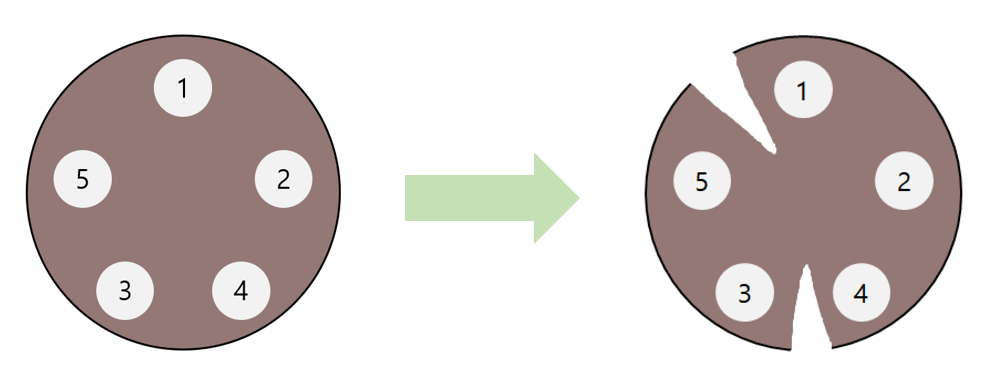
\includegraphics[width=0.4\textwidth]{problems/image/wontak.png}
\end{figure}

위의 그림에서 $1$이 적혀있는 접시를 $1$번 접시라고 한다면, $3$번과 $4$번 접시의 연결을 끊고, $5$번과 $1$번 접시의 연결을 끊어 $[1, 2, 4],\ [3, 5]$의 정렬된 $2$개의 수열을 얻을 수 있다.

원, 탁!을 하는 데에 힘들었던 운동 부족 현빈이는 원, 탁!의 횟수를 최소화하여 정렬된 수열을 얻어내고 싶어 한다. 여기서 정렬된 수열이란, 시계방향으로 보았을 때 오름차순으로 정렬된 수열을 말한다. 원탁에 놓인 접시들의 정보가 주어질 때, 현빈이가 최소 몇 번의 원, 탁!을 하면 원하는 수열을 얻어낼 수 있는지 알아내는 프로그램을 만들어 주자.

\subsection*{입력}

첫 번째 줄에는 접시의 개수 $N(3 \leq N \leq 1\ 000\ 000)$이 주어진다.

두 번째 줄에는 공백을 구분으로 $a_{i}$가 주어진다. $(1 \leq i \leq N;1 \leq a_{i} \leq 1\ 000\ 000)$

\subsection*{출력}

최소 몇 번의 원, 탁!이 필요한지 출력한다.

\subsection*{예제}

\begin{table}[h]
% \centering
\renewcommand{\arraystretch}{1.5}
\begin{tabular}{|L{8.2cm}|L{8.2cm}|}
\hline
\multicolumn{1}{|c|}{\textbf{standard input}} & \multicolumn{1}{c|}{\textbf{standard output}} \\ \hline\hline
% 적절한 예제를 입력하면 됩니다.
\texttt{5} & \texttt{2}\\ 
\texttt{1 2 4 3 5} & \\ 
\hline

\texttt{5} & \texttt{1}\\ 
\texttt{1 2 3 4 5} & \\ 
\hline

\end{tabular}
\end{table}

\newpage

\subsection*{노트}

오름차순 수열이란 뒤로 갈수록 숫자가 커지는 수열을 의미한다.

